\scanpage{132}

Dans cet exemple, on voit tout de suite qu\deleted{e}'il y a sur $C$ une \unsure{contrainte} de commutativité compatible avec les qutres données sss $U$ est commutatif c'est à dire $G$ est commutatif, et que lesdites contraintes correspondent \inserted{alors} aux fonctions $: G\unsure{x|\times}G\handwritten{\unsure{\rightharpoondown|\rightarrow|-}} k^{\handwritten{*}}$ qui sont bilinéaires et antisymétriques. Dans le cas où le $H^{2}(G,k^{\handwritten{\unsure{*|'}}})$ est \inserted{géométriquement} nul (par exemple $G$ cyclique \deleted{et $k$ algébriquement clos}) on voit donc que pour tout choix non nul de $\handwritten{\sigma}$, on a une contrainte de commutativité pour laquelle il n'y a aucun foncteur fibre compatible avec ladite contrainte (et les autres sur aucune extension de $k$. On peut songer à s'en tirer en trouvant au moins des foncteurs fibres gradués compatibles à toutes les contraintes mais on voit déjà que c'est impossible si $k$ de car.deux (où il n'y a p\rlap{q}as de diff\unsure{\rlap{a}é|é}rence entre l'existence de l'un et l'autre type de foncteur fibre, gradué ou non); et sans doute l'analyse doit montrer que l'on a un même résultat négatif en toute caractéristique. Noter cependant dans ces exemples on pouvait au moins, en modifiant la contrainte de commutativité donnée, en trouver une qui admette un foncteur fibre compatible à ladite contrainte. Il y aurait donc lieu de donner un exemple d'une $\unsure{\otimes|\Omega}$-catégorie définissable par une bialgèbre\deleted{\unsure{s}}, admettant une contrainte de commutativité (compatible au reste) mais aucune cont\rlap{a}rainte de commutativité pour laquelle on puisse \rlap{f}t\rlap{o}rouver un foncteur fibre (gradué au besoin)\unsure{;|:}sur aucune extension du corps donné.

\handwritten{Avec les notations du n° 11, il faudra donc 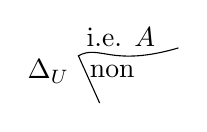
\begin{tikzpicture}[baseline=(du.base),x=1cm,y=1cm]
\node[inner sep=0] (du) at (0,0) {$\Delta_U$};
\node[anchor=west,inner sep=0] at (.52,0) {non};
\node[anchor=south,inner sep=0] at (.92,.31) {\inserted{i.e. $A$}};
\draw (1.65,.3) .. controls (.8,.05) and (.65,.35) .. (.38,.2) -- (.65,-.4);
\end{tikzpicture} commutatif\inserted{\unsure{vu!|u.!}}, et $U$ non commutatif (sinon l'existence de $\sigma$ impliquerait la commutativité de $\Delta$\unsure{]|)}.}
% archive sheet number: 131
